		\begin{question}{N.A.}{Reconnaissance de courbes}{1}{}
			Parmi les différentes représentations de la figure suivante, laquelle représente une évolution périodique?
			\begin{figure}
				\centering
				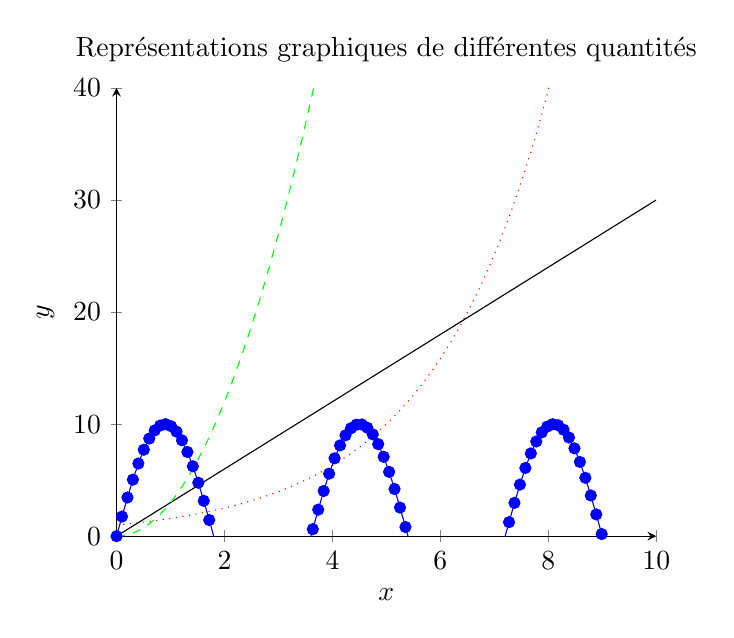
\begin{tikzpicture}
					\begin{axis}[
						title = {Représentations graphiques de différentes quantités},
						axis lines = left,
						xlabel = $x$,
						%minor x tick num = 4,
						ylabel = $y$,
						ymin=0, ymax=40,
						/pgf/number format/.cd,%3 lignes dessous, utiliser spacers français au eu d'anglais.
						use comma,
						1000 sep={\,}
					]
						%Below the red curve
						\addplot [
							domain=0:10,
							samples=100,
							color=red,
							style=dotted,
							%/pgf/text mark = {+}, %changer le marqueur text
							%mark=*,
						]
						{10^(0.2*x)};
						\addplot [
							domain=0:10,
							samples=100,
							color=blue,
							%/pgf/text mark = {+}, %changer le marqueur text
							mark=*,
						]
						{10*sin(100*x)};
						\addplot [
							domain=0:10,
							samples=100,
							color=black,
							style=solid,
							%/pgf/text mark = {+}, %changer le marqueur text
							%mark=o,
						]
						{3*x};
						\addplot [
							domain=0:10,
							samples=100,
							color=green,
							style=dashed,
							%/pgf/text mark = {+}, %changer le marqueur text
							%mark=triangle,
						]
						{3*x^2};
					\end{axis}
				\end{tikzpicture}
			\end{figure}
		\end{question}
		\begin{reponses}
		\item[true] La courbe bleue (cercles).
		\item[false] La courbe rouge (pointillés).
		\item[false] La courbe noire (pleine).
		\item[false] La courbe verte (tirets).
		\end{reponses}
		%%%%%%%%%%%%%%%%%%%%
		\begin{question}{N.A.}{Reconnaissance de courbes}{1}{}
            Parmi les différentes représentations de la figure suivante, laquelle représente une évolution exponentielle?
            \begin{figure}
              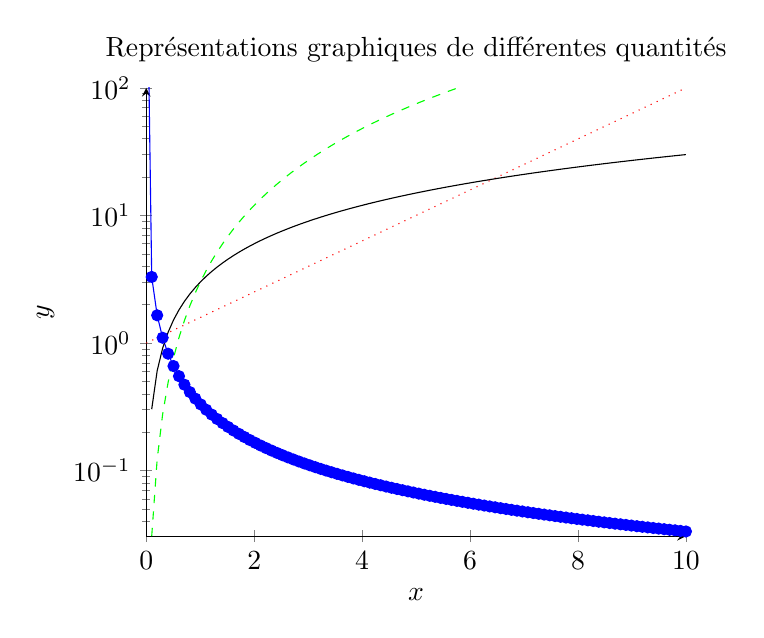
\begin{tikzpicture}
                  \begin{semilogyaxis}[
                        title = {Représentations graphiques de différentes quantités},
                        axis lines = left,
                        xlabel = $x$,
                        %minor x tick num = 4,
                        ylabel = $y$,
                        ymax=100,
                        /pgf/number format/.cd,%3 lignes dessous, utiliser spacers français au lieu d'anglais.
                        use comma,
                        1000 sep={\,}
                      ]
                      %Below the red curve
                      \addplot [
                        domain=0:10,
                        samples=100,
                        color=red,
                        style=dotted
                        %/pgf/text mark = {+}, %changer le marqueur text
                        %mark=o,
                      ]
                      {10^(0.2*x)};
                      \addplot [
                        domain=0.0001:10,
                        samples=100,
                        color=blue,
                        %/pgf/text mark = {+}, %changer le marqueur text
                        mark=*,
                      ]
                      {1/(3*x)};
                      \addplot [
                        domain=0:10,
                        samples=100,
                        color=black,
                        style=solid,
                        %/pgf/text mark = {+}, %changer le marqueur text
                        %mark=o,
                      ]
                      {3*x};
                      \addplot [
                        domain=0:10,
                        samples=100,
                        color=green,
                        style=dashed,
                        %/pgf/text mark = {+}, %changer le marqueur text
                        %mark=o,
                      ]
                      {3*x^2};
                  \end{semilogyaxis}
              \end{tikzpicture}
             \end{figure}
        \end{question}
        \begin{reponses}
            \item[false] La courbe bleue (cercles).
		    \item[true] La courbe rouge (pointillés).
		    \item[false] La courbe noire (pleine).
		    \item[false] La courbe verte (tirets).
		    \end{reponses}
        %%%%%%%%%%%%%%%%%%%%
        \begin{question}{N.A.}{Reconnaissance de courbes}{2}{}
            Parmi les différentes représentations de la figure suivante, laquelle représente une évolution exponentielle?
            \begin{figure}
              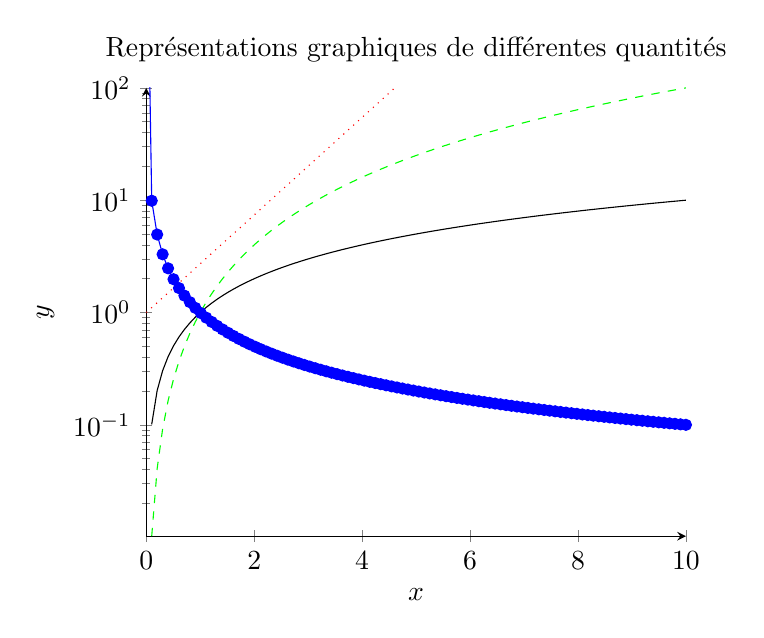
\begin{tikzpicture}
                  \begin{semilogyaxis}[
                        title = {Représentations graphiques de différentes quantités},
                        axis lines = left,
                        xlabel = $x$,
                        %minor x tick num = 4,
                        ylabel = $y$,
                        ymax=100,
                        /pgf/number format/.cd,%3 lignes dessous, utiliser spacers français au lieu d'anglais.
                        use comma,
                        1000 sep={\,}
                      ]
                      %Below the red curve
                      \addplot [
                        domain=0:10,
                        samples=100,
                        color=red,
                        style=dotted
                        %/pgf/text mark = {+}, %changer le marqueur text
                        %mark=o,
                      ]
                      {exp(x)};
                      \addplot [
                        domain=0.0001:10,
                        samples=100,
                        color=blue,
                        %/pgf/text mark = {+}, %changer le marqueur text
                        mark=*,
                      ]
                      {1/x};
                      \addplot [
                        domain=0:10,
                        samples=100,
                        color=black,
                        style=solid,
                        %/pgf/text mark = {+}, %changer le marqueur text
                        %mark=o,
                      ]
                      {x};
                      \addplot [
                        domain=0:10,
                        samples=100,
                        color=green,
                        style=dashed,
                        %/pgf/text mark = {+}, %changer le marqueur text
                        %mark=o,
                      ]
                      {x^2};
                  \end{semilogyaxis}
              \end{tikzpicture}
             \end{figure}
        \end{question}
        \begin{reponses}
            \item[false] La courbe bleue (cercles).
		    \item[true] La courbe rouge (pointillés).
		    \item[false] La courbe noire (pleine).
		    \item[false] La courbe verte (tirets).
		    \end{reponses}
        %%%%%%%%%%%%%%%%%%%%
		\begin{question}{N.A.}{Reconnaissance de courbes}{1}{}
            Parmi les différentes représentations de la figure suivante, laquelle représente une évolution exponentielle?
            \begin{figure}
              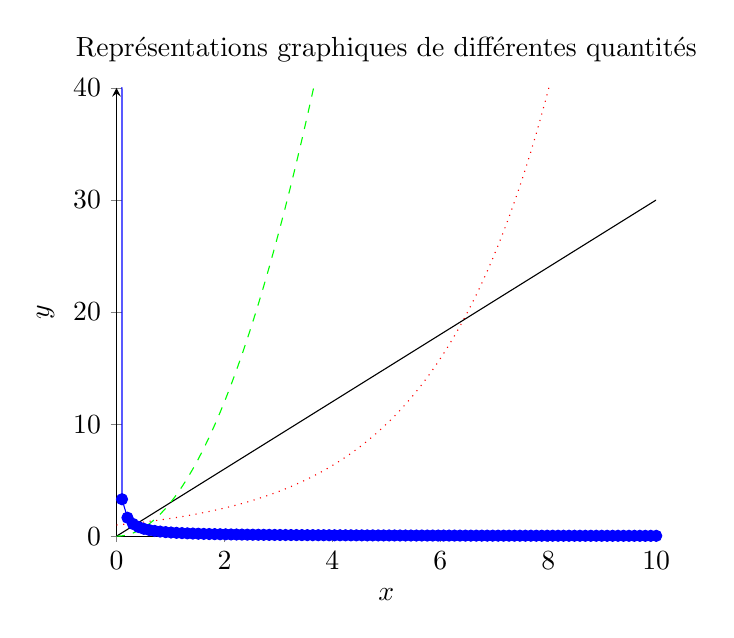
\begin{tikzpicture}
                  \begin{axis}[
                        title = {Représentations graphiques de différentes quantités},
                        axis lines = left,
                        xlabel = $x$,
                        %minor x tick num = 4,
                        ylabel = $y$,
                        ymin=0, ymax=40,
                        /pgf/number format/.cd,%3 lignes dessous, utiliser spacers français au lieu d'anglais.
                        use comma,
                        1000 sep={\,}
                      ]
                      %Below the red curve
                      \addplot [
                        domain=0:10,
                        samples=100,
                        color=red,
                        style=dotted
                        %/pgf/text mark = {+}, %changer le marqueur text
                        %mark=o,
                      ]
                      {10^(0.2*x)};
                      \addplot [
                        domain=0.0001:10,
                        samples=100,
                        color=blue,
                        mark=*,
                        %/pgf/text mark = {+}, %changer le marqueur text
                      ]
                      {1/(3*x)};
                      \addplot [
                        domain=0:10,
                        samples=100,
                        color=black,
                        %/pgf/text mark = {+}, %changer le marqueur text
                        %mark=o,
                        style=solid,
                      ]
                      {3*x};
                      \addplot [
                        domain=0:10,
                        samples=100,
                        color=green,
                        style=dashed,
                        %/pgf/text mark = {+}, %changer le marqueur text
                        %mark=o,
                      ]
                      {3*x^2};
                  \end{axis}
              \end{tikzpicture}
             \end{figure}
        \end{question}
        \begin{reponses}
            \item[false] La courbe bleue (cercles).
		    \item[true] La courbe rouge (pointillés).
		    \item[false] La courbe noire (pleine).
		    \item[false] La courbe verte (tirets).
		    \end{reponses}
        %%%%%%%%%%%%%%%%%%%%
		\begin{question}{N.A.}{Reconnaissance de courbes}{2}{}
            Parmi les différentes représentations de la figure suivante, laquelle représente une évolution linéaire?
            \begin{figure}
              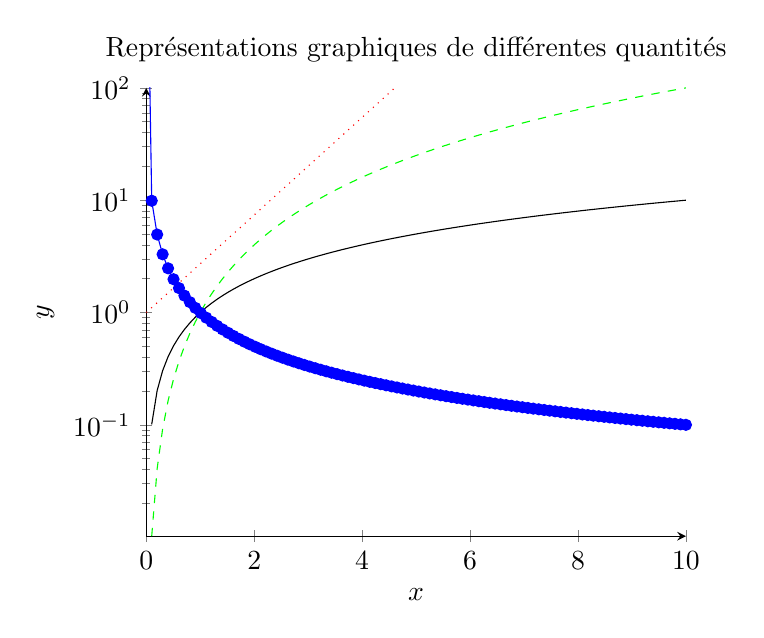
\begin{tikzpicture}
                  \begin{semilogyaxis}[
                        title = {Représentations graphiques de différentes quantités},
                        axis lines = left,
                        xlabel = $x$,
                        %minor x tick num = 4,
                        ylabel = $y$,
                        ymax=100,
                        /pgf/number format/.cd,%3 lignes dessous, utiliser spacers français au lieu d'anglais.
                        use comma,
                        1000 sep={\,}
                      ]
                      %Below the red curve
                      \addplot [
                        domain=0:10,
                        samples=100,
                        color=red,
                        style=dotted
                        %/pgf/text mark = {+}, %changer le marqueur text
                        %mark=o,
                      ]
                      {exp(x)};
                      \addplot [
                        domain=0.0001:10,
                        samples=100,
                        color=blue,
                        %/pgf/text mark = {+}, %changer le marqueur text
                        mark=*,
                      ]
                      {1/x};
                      \addplot [
                        domain=0:10,
                        samples=100,
                        color=black,
                        style=solid,
                        %/pgf/text mark = {+}, %changer le marqueur text
                        %mark=o,
                      ]
                      {x};
                      \addplot [
                        domain=0:10,
                        samples=100,
                        color=green,
                        style=dashed,
                        %/pgf/text mark = {+}, %changer le marqueur text
                        %mark=o,
                      ]
                      {x^2};
                  \end{semilogyaxis}
              \end{tikzpicture}
             \end{figure}
        \end{question}
        \begin{reponses}
            \item[false] La courbe bleue (cercles).
		    \item[false] La courbe rouge (pointillés).
		    \item[true] La courbe noire (pleine).
		    \item[false] La courbe verte (tirets).
		    \end{reponses}
        %%%%%%%%%%%%%%%%%%%%
